\documentclass{ucthesis}

% Image support with PDF conversion
\usepackage[pdftex]{graphicx}
% Inserts a line feed between paragraphs, because it makes me feel grown up
\usepackage{parskip}
% Underline text using \uline{...}
\usepackage[normalem]{ulem}
% Sane URL handling
\usepackage{url}
% Math equations
\usepackage{mathtools}
% source code typesetting
\usepackage{algpseudocode}
\usepackage{listings}
% Include an appendix!
\usepackage{appendix}


\begin{document}
\title{Examining Ambiguities in the Automatic Packet Reporting System}
\author{Kenneth W. Finnegan}
\degreemonth{December} \degreeyear{2014} \degree{Master of Science}
\defensemonth{November} \defenseyear{2014}
\numberofmembers{3} \chair{Bridget Benson, Ph.D.} 
\othermemberA{John Bellardo, Ph.D.} \othermemberB{Dennis Derickson, Ph.D.}
\field{Electrical Engineering} \campus{San Luis Obispo}
\maketitle

\begin{frontmatter}

\copyrightpage
\committeemembershippage

\begin{abstract}
The Automatic Packet Reporting System (APRS) is an amateur radio packet 
network that has evolved over the last several decades in tandem with, 
and then arguably beyond, the lifetime of other VHF/UHF amateur packet
networks, to the point where it is one of very few packet networks left
on the amateur VHF/UHF bands. This is proving to be problematic due to
the loss of institutional knowledge as older amateur radio operators who
designed and built APRS and other AX.25-based packet networks abandon
the hobby or pass away. The purpose of this document is to 
collect and curate a sufficient body of knowledge to ensure the 
continued usefulness of the APRS network, and re-examining 
the engineering decisions made during the network's evolution to look for
possible improvements and identify deficiencies in documentation of
the existing network.
\end{abstract}

\tableofcontents
\listoffigures
\end{frontmatter}

\chapter{Preface}

Like any major research endeavor, this thesis certainly didn't start anywhere near
where it ended.
Most of the credit for the genesis for this thesis needs to be given to 
Sivan Toledo, 4X6IZ, from Tel-Aviv University. In 2012 he wrote an article in the
amateur radio QEX technical journal where he explored improving the soundcard 
digital signal processing modem used for amateur packet radio by passing the 
original signals through a series of band-pass filters \cite{sevanhighperf}. 
His improvements were
commendable, and his article was very well written, but what bothered me was that 
more than three decades after the inception of amateur packet radio,
we are still seeing
measurable improvement in the modems we use for the original modulation techniques.

This thesis started with me wanting to tear apart the current state of the various
Bell 202 modems used in amateur radio, build a quantitative model of the kinds of
interference and distortion that each modem handled well, and hopefully design
a new signal processing algorithm that showed immunity to the most common forms of
interference on real-world channels. Sevan's work in JAVA showed promise, but 
while his library is useful on desktop computers and Android devices, it left 
out in the cold the many different 8, 16, and 32 bit fixed-point microcontrollers
that are often used for embedded modems in amateur radio projects.

As I started to examine the specifications for the various network layers used
in the amateur Automatic Packet Reporting System (namely Bell 202, AX.25, and
APRS), I grew increasingly shocked and confused when I kept finding that the
documentation I was looking for was poorly written or simply didn't exist. 
Protocol specifications would identify variables critical for network performance,
and then never give guidance on what the actual value should be.
Many of the documents
on the expected behavior for network nodes consist solely of console commands
to be run on specific pieces of discontinued hardware instead of actual protocol
behavior.
Most articles discussing aspects of the network disagreed with 
other documentation on specific details,
and was often internally inconsistent as well.

The final turning point was an interview in March, 2014 with Scott Miller, the
designer for Open Trackers, 
which are one of the more popular lines of contemporary modems used in the APRS
network.
I brought a laundry list of inconsistencies from the network specs and he
explained how much effort he had put into reverse engineering the existing 
hardware. It was an eye-opening conversation that drove home how much the 
amateur packet network has grown haphazardly over the past three decades into
a jumble of band-aids applied upon band-aids.

I realized that the most important academic research on the topic of APRS isn't
how to squeeze out another incremental improvement in one of the modem DSP
algorithms, but an over-arching prolegomenon on the entire network stack as it 
actually exists today. The existing documentation clearly falls short, and
much of the institutional knowledge that I've been able to draw on during 
my research is coming from the ``old guard" of the hobby, which leaves us exposed
to the labor intensive requirement of newcomers to the network to 
reverse engineer the existing network before they can participate.

Ideally, this document would be able to stand by itself as a complete 
``implementer's guide to APRS" from the physical layer all the way up to high level
aggregate network behavior, but the scope of reverse engineering that much
behavior, documenting it, and then verifying the documentation quickly becomes
monumental. 
It is my hope that this document does at least identify the most glaring 
short-falls in the current documentation and network design, and gives answers to
the questions that can be answered while staying within the scope of this survey.

For every identified problem which is answered in this paper, there
are twice as many unanswered questions which each warrant being considered 
as a thesis of their own.


\chapter{Introduction}

The Automatic Packet Reporting System (APRS) is an amateur radio packet
network designed to provide each participating node a local view of the 
tactical environment based on each node beaconing it's current status
and advertising any other local resources known to exist.

Exactly what types of resources should be advertised on a local APRS
network is left to the discretion of the local network coordinators, but
a typical APRS network would advertise information such as:
\begin{itemize}
\item The location of amateur radio operators and what frequencies they are using for voice communications.
\item The location, frequency, and access information for voice repeaters
\item The location and status of APRS digital repeater nodes
\item The location and access information for other packet networks such as BBSes, Winlink nodes, or open Internet access points.
\item The location and status of useful facilities such as rest stops, resupply points for food/water, etc.
\item Telemetry from sensors such as weather stations or remote site monitoring (i.e. battery voltage at solar sites)
\item Short real-time messages and announcements directed at other amateur radio operators
\end{itemize} 

Despite these flexible capabilities, 
and much to the chagrin of many of the original designers of APRS, 
the vast majority of user traffic on the APRS network consists solely of 
real-time automatic vehicle tracking (AVT).
Fittingly, it follows that one of the hotbeds for APRS network congestion
is the Los Angeles basin, 
due to its bowl-shaped geography and unusually high population density.
When discussing specifics of the APRS network, such as how often to send traffic
or how many hops to route it over, LA invariably comes up as a counter-example
that under-cuts any specific guidance on what to expect from the network.

The author is more interested in being able to make concise statements about 
APRS in general than construct an entirely exhaustive analysis, 
so the reader need only appreciate that places like LA are the exception to the rules.
Any readers operating in the LA basin have the author's heart-felt condolences,
but need look elsewhere for definitive guidance on operating in such a unique
part of the APRS network.

\section{History of APRS}

APRS was created as an evolution of the AX.25 packet networks
built throughout the amateur community during the 1980s and 1990s and 
the Connectionless Emergency Traffic System (CETS) built by 
Bob Bruninga during the early 1980s to map Navy position reports.

Near-ubiquitous access to the Internet caused the decline in local BBS 
systems and AX.25 TCP/IP networks during the 1990s, but APRS has 
continued to enjoy a growing user-base due to it filling a unique 
application of amateur packet radio to local short-lived communication.
The 1200 baud Bell 202 modems used for AX.25 are often bemoaned for having
such a low data rate, but proves to be plenty of bandwidth for the short periodic
text messages involved in APRS.

APRS supports basic communication between stations via node to node 
text messages and comment field status updates, but should not be 
considered a communications network to an end, but a way to be made aware
of the other assets in the local area made available to support amateur 
radio operations.

Due to the fact that APRS is built upon the relatively slow 
1200bps AX.25 VHF packet
network and the channel sharing concepts developed for the ALOHAnet at
the University of Hawaii, the amount of 
traffic and the number of stations that it is possible to successfully 
support on a single regional network is severely limited. 
A typical APRS network is considered successful if a single node
can use it to discover the 60 closest other assets on the network in a
10-30 minute time frame. Trying to advertise information beyond this
``ALOHA circle" consisting of the 60 closest stations exceeds the 
operational objective of the APRS network and usually proves to only be 
detrimental to the network and other users as network throughput is 
consumed by advertisements for 
resources beyond the radius of interest for the local operator.

\section{Physical Topology and Hardware}

A typical APRS network consists of three types of stations:
\begin{itemize}
	\item Trackers - These are mobile radios, often installed in vehicles with
		a GPS receiver, that periodically advertise their physical location
		along with any additional information including what other frequencies
		the operator is listening on.
	\item Digipeaters - These are half-duplex digital repeaters that build the
		backbone of an APRS network, allowing stations to interact with other
		stations beyond their immediate radio range. This is done by immediately
		repeating any received packets which request being repeated from the
		digi's higher location.
	\item I-gates - Internet gateways are stations usually installed in homes
		that act as bridges between the local APRS network on RF and the
		world-wide APRS-IS (Internet System) network, which uses the Internet
		to aggregate and route all of the APRS traffic generated in each
		local network to one unified network.
\end{itemize} 

As each tracker beacons its information for the local network, it is repeated
by the digipeaters for consumption by other local stations, and gatewayed
to the Internet by any I-gates that receive the packet along the way. 
Figure \ref{fig:demonetwork}
shows the typical path of a packet from a low-powered handheld tracker as it moves
throughout the local APRS network. It's not unusual for battery-powered trackers to
only output one to five watts of RF power, which limits their range to any stations
immediately around them. 
Since digipeaters are often higher power with 
high-quality antennas, them repeating packets from these low-power trackers 
greatly increases their range and usefulness.

\begin{figure}
	\centering
	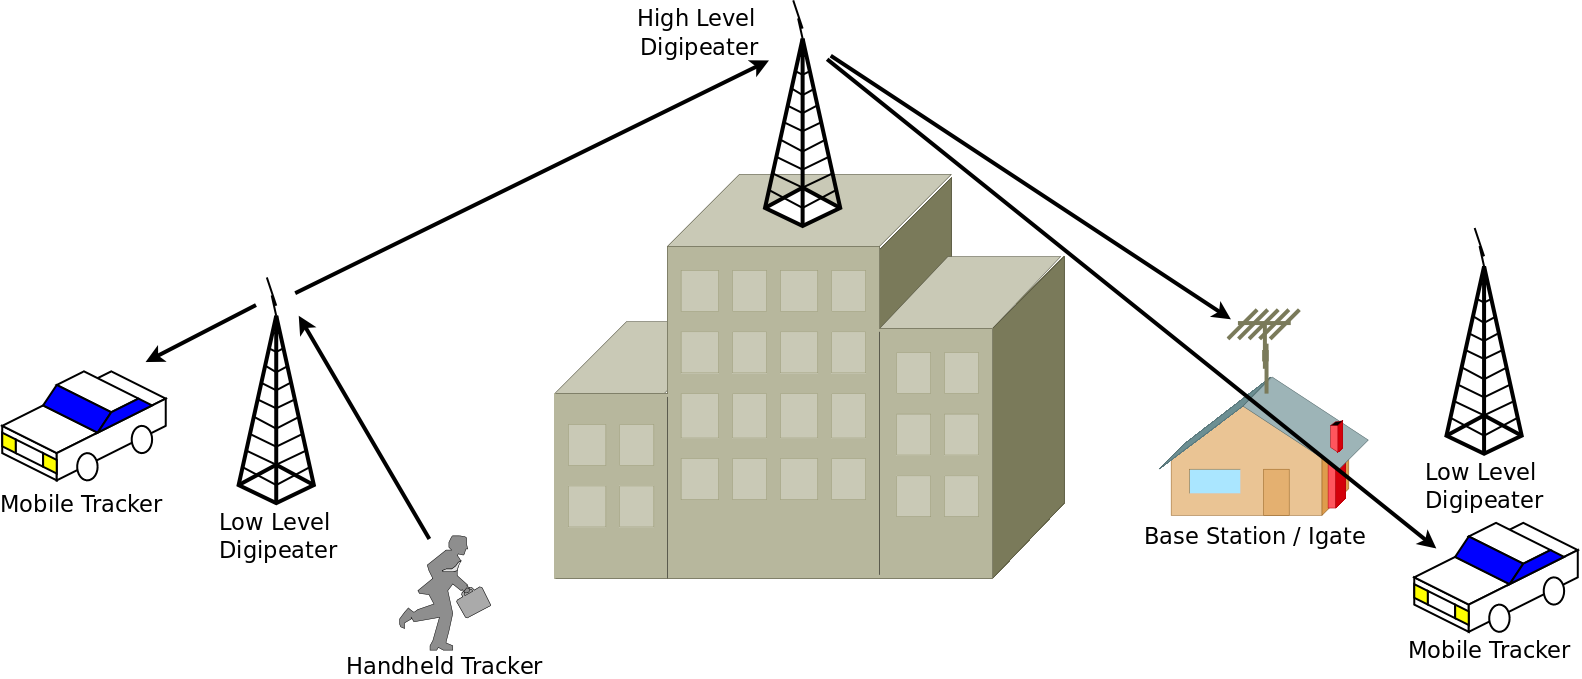
\includegraphics[width=1.0\textwidth]{src/dia/demonetwork}
	\caption{Example packet path from a handheld APRS tracker}
	\label{fig:demonetwork}
\end{figure}

\subsection{Station Block Diagrams}

Like most aspects of the APRS network, there are countless options 
when it comes to assembling an APRS node from the parts on-hand.
This section presents block diagrams for the three most common ways
to assemble trackers, digipeaters, and I-gates, but additional permutations
of these and entirely different topologies are possible.

Blocks presented as dotted lines are optional. The ``Transceiver" blocks refer to 
VHF FM amateur radios. ``Terminal Node Controllers" are the modems and radio
interfaces with minimal embedded intelligence. These blocks and the labeled protocols
between blocks will be expanded upon in later chapters.

\begin{figure}
	\centering
	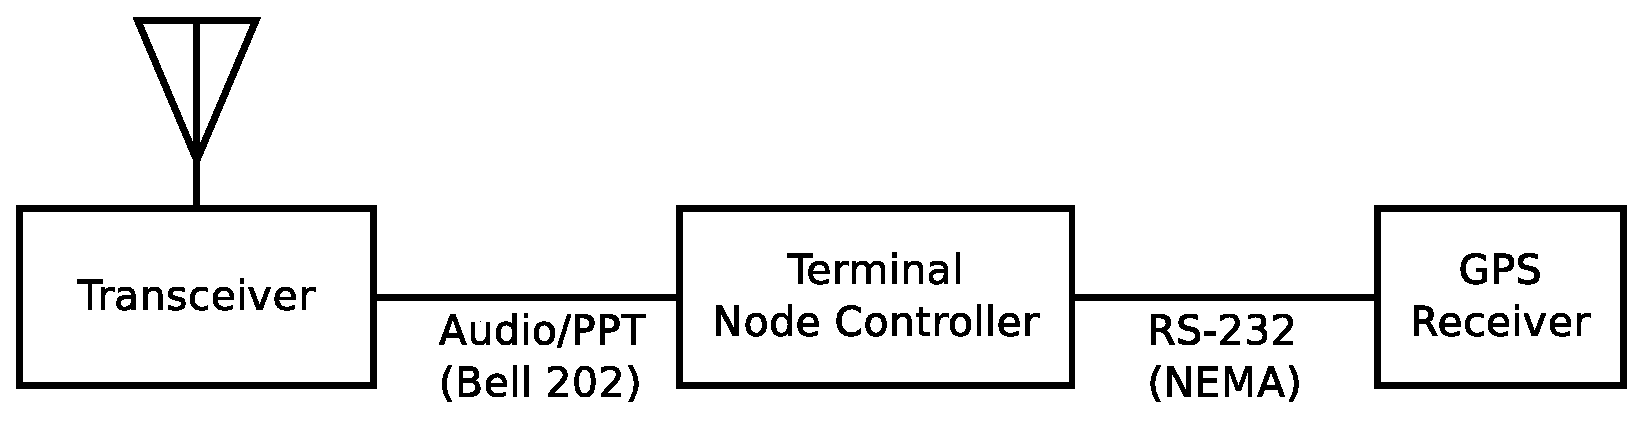
\includegraphics[width=0.7\textwidth]{src/dia/tracker}
	\caption{Block diagram for typical APRS tracker}
	\label{fig:blocktracker}
\end{figure}

Figure \ref{fig:blocktracker} shows the block diagram for an APRS tracker, 
which is built around a Terminal Node Controller which parses NEMA positions
provided by a GPS receiver and convert them into APRS position reports that
are then frequency shift modulated and sent to a VHF FM voice transceiver using an
interface cable that includes transmit and receive audio, as well as a line to
key the ``push to talk" button on the radio to start transmitting.

\begin{figure}
	\centering
	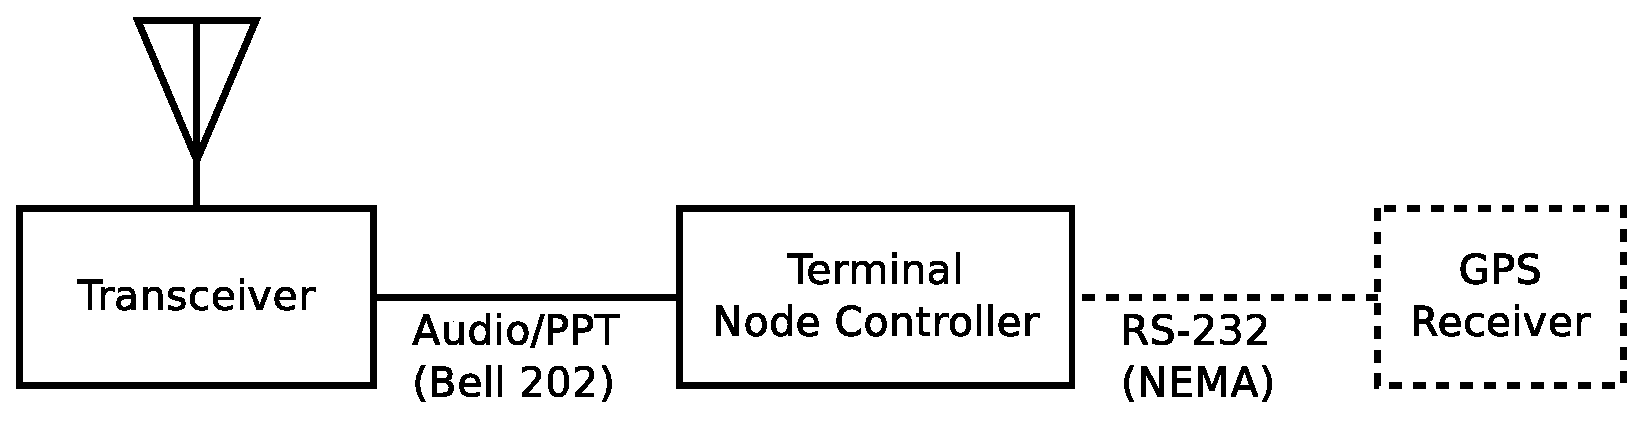
\includegraphics[width=0.7\textwidth]{src/dia/tnc_digi}
	\caption{Block diagram for typical APRS Digipeater}
	\label{fig:blockdigi}
\end{figure}

Figure \ref{fig:blockdigi} shows the block diagram for a digital repeater, which
is much the same as for a tracker except that the GPS receiver is often omitted. 
Since the digipeater is always installed in a fixed location, its GPS coordinates
can be hard-coded into non-volatile memory in the TNC.

\begin{figure}
	\centering
	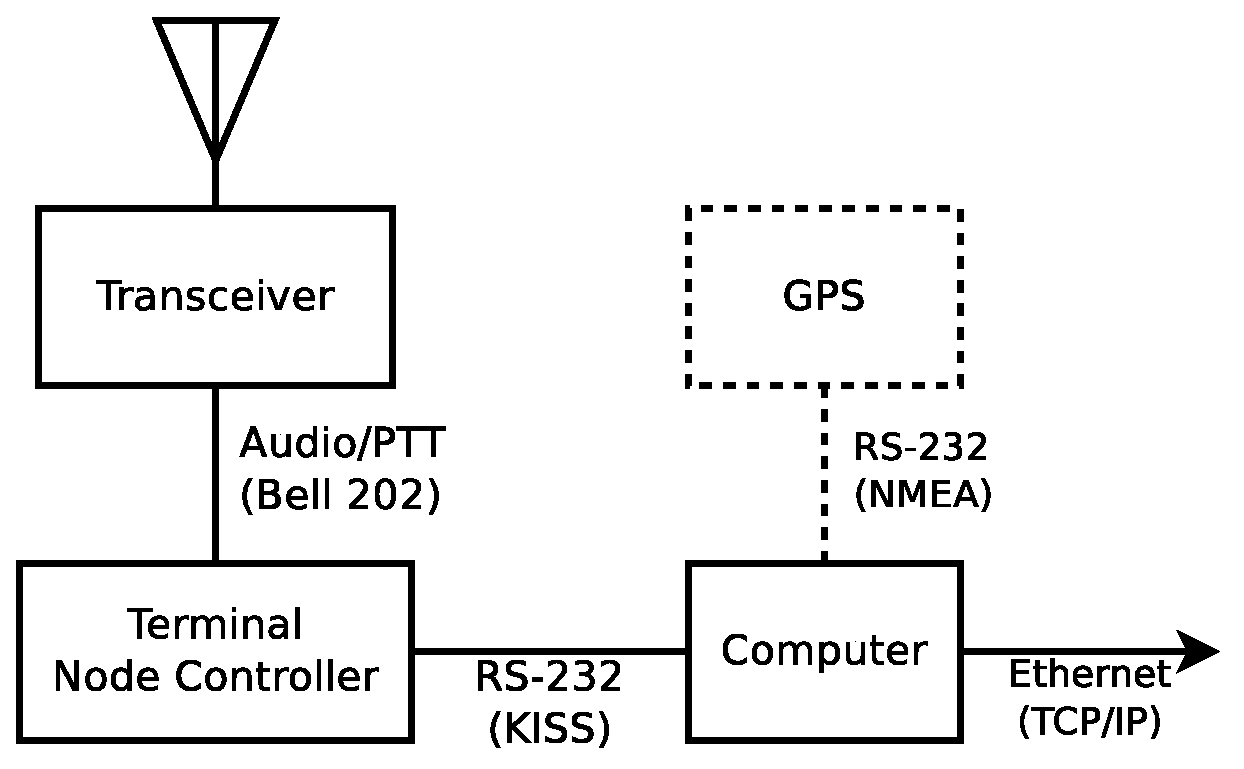
\includegraphics[width=0.7\textwidth]{src/dia/igate_kiss}
	\caption{Block diagram for typical APRS Internet Gateway}
	\label{fig:blockigate}
\end{figure}

Figure \ref{fig:blockigate} shows the block diagram for an Internet Gateway, which
like the digipeater doesn't require a GPS receiver. Unlike the digipeater,
instead of sending received packets back out through the VHF transceiver,
I-gates send received packets to the APRS-IS Internet System via a local connection
to the Internet.


\section{Document Overview}

The rest of this document is going to start at the bottom of the APRS protocol
stack and work its way up, touching on each layer with an introduction and
some basic analysis. 
Ideally, this document would answer all of the ambiguities existing in the
APRS network protocols, but many of the issues that will be touched upon 
deserve an entire masters thesis of their own, and therefore will only
be noted as currently deficient. 
Any readers still shopping for a thesis subject or senior project should 
continue reading with bated breath, as this topic is ripe with further 
work.

Part \ref{part:physical} will cover the Bell 202 modem used to encode APRS on
the VHF packet channels and the KISS protocol used to connect modems to
host devices such as computers. Chapter \ref{chap:bell202} will go into an
unusual amount of detail since a specification document for Amateur Bell 202
was never written and therefore will likely prove to be one of the more significant
contributions of this paper to the field.

Part \ref{part:datalink} will touch on what could be called the data link layer
of APRS. It will start with an introduction to the concept of a terminal
node controller, move into how the AX.25 protocol has been modified for APRS, and
finally discuss the digipeater behavior needed to flood packets from their
originating stations throughout the network.

Finally, part \ref{part:network} will discuss the popular algorithms used to 
determine how and when an individual node should send packets to the network,
and introduce some simple models for the 
expected capacity of a typical APRS network.


\part{OSI Layer 1 --- Physical}

The physical layer of APRS defines the different signalling methods used
to transport datalink layer packets from one node to another across one of
the several physical channels typically used in the APRS network.


\chapter{Bell 202 on RF}

The most common layer 1 used for APRS on RF is a variant of the
Bell 202 audio frequency shift keyed (AFSK) modem transmitted via 
FM VHF radios. In North America, the primary frequency of operation is
144.390MHz, but differs by country based on local band limitations.

Bell 202 was originally  based on switching between 1200Hz and 2200Hz tones to
represent a binary one or zero respectively. Due to Amateur radio operators
using Bell 202 as a physical layer below AX.25, which ultimately derived 
from HDLC, the original 1200Hz mark and 2200Hz space symbols are not used;
the layer 2 data stream is encoded using 
non-return to zero, inverted (NRZI),
which requires zeros in the original bit stream to be encoded as a change
between 1200Hz and 2200Hz and ones to be encoded as transmitting the same
symbol during the next symbol period as during the prior.

\section{Stages of a Bell 202 Transmission}

Channel idle state; string of zeros for clock sync

At least one flag octet 0x7E

AX.25 UI frame with bit stuffing

Frame Check Sum; 16 bit CCITT CRC

At least one flag octet 0x7E

Release of channel or an additional AX.25 frame and flag. 

\section{Baseband Performance of Bell 202 Modems}

TODO No FEC is severe limitation

TODO Emphasis / deemphasis problem is unsolvable

TODO Define Basic 3002 phone channel as good benchmark

\section{Carrier Sense Multiple Access}
\label{sec:bell202csma}

Since amateur Bell 202 is a half duplex modulation traditionally using FM voice 
transceivers, one of the challenges to packet radio is avoiding multiple stations
transmitting on the same channel at once. Other derivatives of ALOHAnet, such as 
the original half duplex 10Mbps Ethernet, have the advantage that transmitters can
at least sense when a collision has taken place and use that information to abort
the transmission of the rest of the frame.

Throughout the history of APRS, there has been several debates as to the implications
of CSMA algorithms and primarily the need for one at all versus an entirely 
stocastic channel access method. The argument follows that the majority of 
channel contention is between multiple clients trying to reach a single digipeater
across what's called a split horizon, where each of the clients can hear and be heard
by the digipeater, but are entirely unaware of each other. In these types of instances,
even an optimal CSMA algorithm will never correctly cause one of the stations to hold 
off until the end of the other's transmission due to the needed information being
entirely unavailable.

Besides the degenerate case of ignoring the current channel status completely when 
deciding to transmit a pending frame, there are two major algorithms used for CSMA;
DWait and P-persistent.

DWait is a deterministic algorithm where each station is assigned a fixed
``quiet time" after the end of another tranmission before they will begin a locally
pending tranmission. This lends itself well to very carefully designed networks
where the relative priority of each station is known and a corresponding DWait time
is set for each station where a shorter DWait will always gain the channel over a longer
one. The requirement for the network to have an overarching design doesn't lend itself
well to the national APRS network, but could be applied effectively for localized 
portions of the APRS network and for ``insular" networks built for special events or
private groups of amateurs.

P-persistent is a statistical algorithm with two variables: the slot time, and the
probability that a station should transmit at the beginning of a slot. The slot time
should presumably be set to as short of a time interval during which a station can
reliabily identify another station as transmitting before beginning its own transmission,
and the P value for how likely a station is to transmit should be set based on the 
number of other stations with pending traffic attempting to gain the channel.

TODO Table of typical mobile radio tx-rx and rx-tx changeover times.
TODO The typical 100ms slot time seems to be much too short.

\chapter{KISS}

During the early 1980's when amateur Terminal Node Controllers were developed,
the expectation was that the TNC would be handling 
the entire packet protocol stack up to the final presentation to the user, which
could be done using a dumb terminal such as a VT100 or line printer 
and a keyboard. 
As personal computers became affordable in the late 1980's, the expectation that
the entire application stack would run on the embedded TNC became severely limiting
and KISS (``Keep It Simple, Stupid") emerged as the solution to 
expose the modem inside TNCs via 
an eight bit clean interface and bypass the TNC's internal network stack.

KISS was originally presented by 
Mike Chepponis, K3MC and Phil Karn, KA9Q at the 6th ARRL Computer Networking
Conference in Redondo Beach, CA \cite{KISSspec}.
KISS was designed as an extension to the Serial Line 
Internet Protocol (SLIP) allowing for in-band signaling from 
the host to the TNC to enable setting modem 
configuration parameters such as the preamble length and CSMA parameters.

This meant that the existing TNCs with their radio interfaces could
be upgraded once with new ROMs that supported KISS and any new network behavior
or protocol could be instead implemented on a seperate host PC.
This was particularly valuable since personal PCs were much
more productive development environments than the 256kb EPROMs and 8 bit
Z80 microprocessors of the popular Tucson Amateur Packet Radio TNC 2 product
and it's several clones \cite{TNC2manual}.

\section{Isolating Modulation from Network}

The advantage of KISS is that it has become the standard packet interchange protocol
between TNC modems and host network controllers,
enabling each side to experiment with new protocols.
This means that as the APRS protocol has evolved, stations that used the
KISS protocol are able to continue using the same ROM-based modems and only
need to upgrade the software running on their host system.
This abstraction holds up even further in that it allows operators to
use different data link protocols than AX.25,
yet there have been few examples of this since the collapse of the IPv4 amateur
radio networks with the wide-spread deployment of the Internet.

As discussed in the prior chapter,
as Bell 202 and HDLC begin to show their age, the field is ripe for a new
modulation to replace them on VHF/UHF packet networks.
Should a researcher wish to deploy a new modulation to use under APRS,
all that needs to be done is build new KISS modems, which will seamlessly
interface with most existing APRS software.
Replacing Amateur Bell 202 modems has always been a popular subject of
discussion on the APRS mailing lists, and is an area ripe for future
quantitative study.

\section{Shortcomings of KISS}

While originally presented as an interim solution until a better protocol was
developed, KISS has enjoyed a lasting popularity among its users.
One concern about KISS that has spawned several derivative protocols is the
lack of a checksum used in each KISS frame.
Should any bit errors happen between the host system and the modem,
they may go undetected and cause corruption in the transported payload
as it continues through the network.
One of the most popular of these derivatives of KISS is SMACK (Stuttgart Modified
Amateurradio-CRC-KISS), which is a backwards compatible extension to KISS
which includes a frame checksum to protect against frame corruption \cite{smack}.

Traditionally, KISS links between the host PC and KISS modems have been deployed
over relatively short RS-232 serial links (three to six feet),
though an increasing number of modems are moving to a pure USB implementation.
What the author has been unable to find is any evidence that when correctly
deployed that these types of short serial links stand any risk of corruption
which could be avoided by using the SMACK extension.
Further study is needed to examine typical APRS KISS deployments to justify
the additional effort required to implement and deploy SMACK above KISS to
protect against any possible corruption risks.

A second shortcoming of KISS which has not evoked anywhere near the
level of discussion that the corruption issue has is KISS' lack of any way
for modems to pass out-of-band (OOB) information back to the host PC.
KISS defines numbered command codes for the host to pass information to the
modem, including channel access settings and hardware specific settings
beyond the type `0' data frame that should be transmitted on the channel.
In the opposite direction, from modem to host, the KISS specification explicitly
limits frame types to only data frames.
This disallows hosts from being able to interogate modems as to their
current configuation settings or any information about the RF channel
beyond packets as they are received.

The author suggests that a revision to the KISS specification be considered
that would allow modems to pass non-zero payloads back to the host PC.
Legacy applications would need to properly discard these non-zero frames
as OOB data that they are not interested in,
while enabling new applications such as interactive configuration programs
and give more meaningful metrics as to current channel utilization.
\begin{itemize}
	\item An interactive configation program would allow a user
		to request a dump of the current configuration, edit it, and
		re-upload it to one or several KISS modems. A canonical example
		of this type of application is the OTWINCFG tool 
		provided by Argent Data for their trackers \cite[\S17.6]{ot3manual}.
	\item Channel utilization information could include how much time
		is consumed on the channel by AFSK data that does not decode as
		valid packets. Some APRS applications attempt to estimate channel
		utilization based on received packets, which will consistently
		under-estimate the actual figure due to frame preambles
		and frames which fail their checksums never being reported.
		The worst case of continuous collisions would result in
		the application misinterpretting no received packets as
		an entirely idle channel, where the opposite is the actual case.
\end{itemize}

\section{Conclusion}

KISS have proven itself tremendously useful as it has decoupled the modem
hardware from the network protocol used above it.
The decreasing price and size of single-board computers such as the
BeagleBone have cemented the popularity of network nodes built using
a full-fledged computer that uses a KISS modem as a radio interface.
It should be appreciated that KISS enables the development of new
modulation schemes without the need to modify existing APRS software
to run over new higher-quality links.
Future work involving KISS should involve studying the quanitative risks
of not using checksums on the serial link between the host and the modem
and the feasibility of extending KISS to allow OOB information to be passed
from modem to host.



\chapter{Bell 103 and PSK63}

TODO Mention the two main HF modes. 


\part{OSI Layer 2 --- Data Link}
\label{part:datalink}


\chapter{AX.25}

AX.25 is the amateur radio derivative of CCITT X.25 that was designed during the early 1980's 
as the primary data link protocol used by amateur packet networks.
The AX.25 specification has been maintained by the Tucson Amateur Packet Radio (TAPR) 
organization until its latest release, Version 2.2 in July of 1998. 

The most significant difference between AX.25 and the original X.25 protocol lies
in the hardware addresses used by AX.25, which are based on the expectation of
each station using their FCC-issued callsign. 
Each node is addressed by their callsign plus an additional 4 bit 
secondary station identifier (SSID), which allows each licensee to maintain and operate 
up to 16 stations in each packet namespace.

AX.25 is one of the best-documented protocols used in amateur radio packet networks,
so it could be argued that a chapter in this thesis considering AX.25 could be omitted.
The AX.25 specification goes into tremendous detail as to the expected behavior of each
node and how the system should transition between states.
Where the documentation does fall short is in how APRS abuses a small subset of 
the AX.25 protocol for the specific needs of the APRS network.
The rest of the chapter will walk through each field of the AX.25 packet and
note how it is used by APRS, followed by a discussion of the implications of the FCC
requirement to identify an active transmitter by its FCC-issued license every ten minutes.

\section{Header Format for APRS}

A very limited subset of the complete AX.25 protocol is used by APRS due to APRS 
deliberately avoiding the use of any of the connected or control modes of AX.25. This 
means that any AX.25 protocol stack used for APRS need only support Unnumbered Information (UI)
frames, and many APRS protocol stacks cannot handle any other forms of AX.25 traffic. 
Figure \ref{fig:ax25uiformat} presents the modified form of the AX.25 frame that is used
by APRS.

\begin{figure}
	\centering
	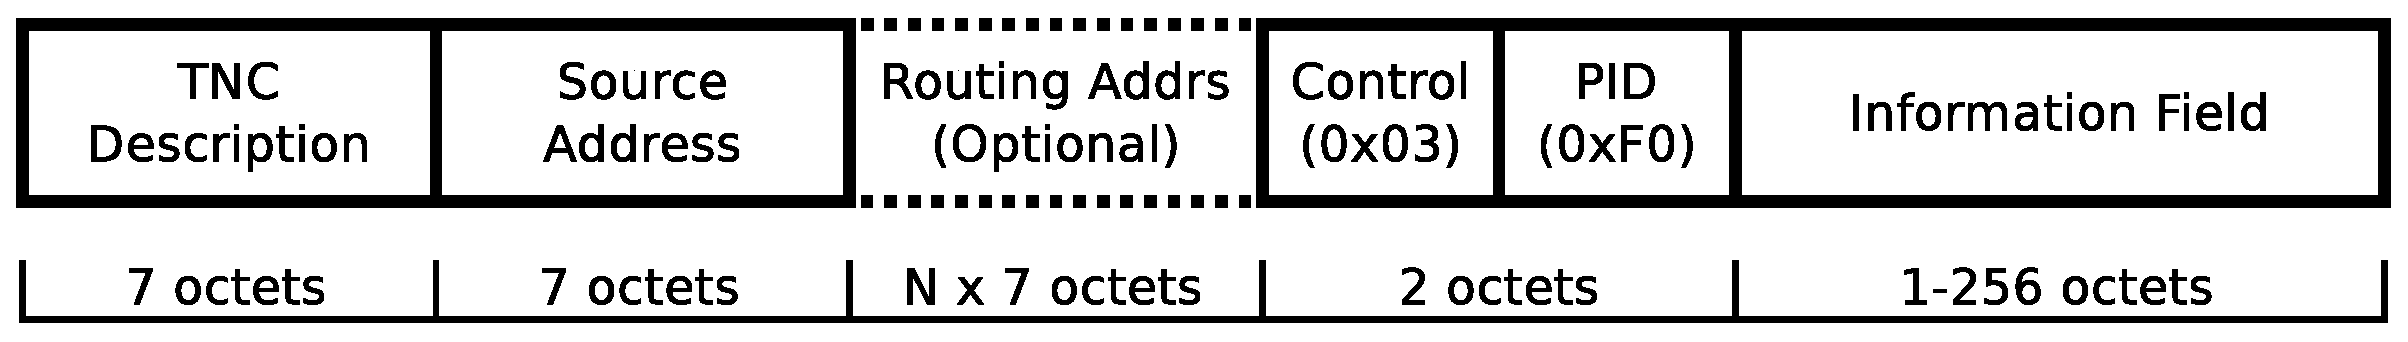
\includegraphics[width=1.0\textwidth]{src/dia/ax25ui}
	\caption{AX.25 UI Packet Format}
	\label{fig:ax25uiformat}
\end{figure}

\subsection{TNC Description / Destination Address}

Traditional AX.25 traffic is usually directed at a single station, which would be indicated by 
a packet's destination address. 
Since APRS is strictly a one-to-many network protocol at layer 3, this field
was deemed not needed for APRS and several alternative uses for the field have been proposed.

The most popular application for this field is to be used as a tracker identifier, where a
six character identifier is allocated from the APRS Working Group to identify a specific 
APRS TNC and firmware version. 
This provides valuable information to the rest of the APRS network.
APRS
TNCs often ``misbehave" and it is helpful to be able to immediately identify the original
developer for a remote APRS node. 
Experimental trackers which have not yet received a tracker ID may use the 
APZ prefix with three additional arbitrary alphanumeric characters as their TNC identifier.

\subsection{Source Address}

The source address is either the FCC-issued or a ``tactical" callsign used by 
the beaconing APRS station, with an 
additional SSID appended to the station, which may range from zero to 15. Source addresses must 
be at least three characters long, and may not be any longer than six. Stations using AX.25 
over RF are limited to the SSID's of 0 to 15 due to AX.25's binary format, 
while APRS imposes a looser standard such that the SSID is only limited to 
two alphanumeric characters.

\subsection{Routing Path}
\label{subsec:ax25RoutingPath}

The AX.25 routing path is an optional variable-length field consisting of an ordered list of
digipeaters which should process and re-transmit the considered packet. Should a station not
require the use of this field, it can be completely omitted and the end-of-path bit should be
set on the source address field. The path must consist of an integer number of seven octets.

The original AX.25 version 2.0 spec allowed for anywhere from zero to eight digipeaters to
be included in an AX.25 frame. Unfortunately, due to the unreliable nature of amateur 
packet radio, packets with a routing path requesting as many as eight hops would rarely be 
successfully delivered to the end station.
The version 2.2 specification for AX.25 was
rewritten limiting the number of requested digipeaters to two with the argument that packets
traveling beyond two hops should be handled by a higher layer protocol than AX.25.
Because AX.25 doesn't guarantee delivery from a digipeater to another station,
packets passing through a digipeater that are lost need to be
resent from their origin.
Higher layer protocols can recover from a lost packet locally 
without needing to twice consume
the bandwidth used to get the packet to the digipeater.

This concept of higher-layer retries and limited digipeater use is ignored by APRS.
More than two digipeater fields are often seen on APRS traffic, 
and users are only strongly discouraged from using a large number of hops.

\subsection{Control Flags}

The Control Flag octet indicates different modes for the AX.25 frame.
Since APRS strictly uses only Unnumbered Information (UI) frames, this field must
contain the value 0x03.

\subsection{Protocol IDentifier}

The Protocol IDentifier (PID) field is normally used to identify the Layer 3 protocol
being transported by AX.25. TAPR has reportedly stopped processing requests for new PID
values to be issued to new layer 3 applications of AX.25 \cite{millernopid}, 
which is a possible explanation for why APRS doesn't have a unique PID.
It instead uses the value of 0xF0, incorrectly indicating that no layer 3 protocol is in use.

\subsection{Information Field}

The rest of the AX.25 frame contains the APRS payload in
what is called the Information Field.
The end of the Information Field is indicated by the Layer 1 modulation, which is traditionally
the Amateur Bell 202 FCS and 0x7E flag.

The maximum transmission unit for the Information Field is 256 octets, and APRS imposes
a minimum of one octet identifying the type of APRS packet being carried \cite{aprsspec}.

\section{FCC Identification Requirements}

One of the conditions of operating a radio under FCC Title 47 CFR Part 97 is that amateur radio 
operators are required to transmit their callsign at least once every ten minutes during an exchange.
An ongoing source of controversy in the APRS community is what this means for operating
an APRS node, and particularly digipeaters.

The source of argument is what constitutes properly identifying the
transmitting station; only a station's FCC callsign in the source address field,
or simply including the callsign somewhere in the complete frame.
Considering only the source address field as a valid way to identify a station is
a very conservative interpretation of \S97.119, but establishes the requirement that every 
digipeater active in the APRS network needs to originate a new packet every ten minutes.
Alternatively, accepting the digipeater's callsign injected anywhere in an outgoing 
packet lends itself to the digipeater staying more ``quiet" since appending its callsign
to the end of the routing path of incoming packets could be considered identification enough.

The considered disadvantage of the more conservative interpretation is that the additional
beacons being generated by every active digipeater every ten minutes is an
excessive burden on the APRS network. Digipeaters rarely have information of value
to the rest of the APRS network, so their beacons are seen as little more than noise.
This interpretation also prohibits the use of ``tactical" callsigns, which are selected
to convey more useful information that the control operator's callsign.
One common example is digipeaters on major mountain peaks; a digipeater 
on Tassajara peak beaconing as ``TASS" has a more meaningful name than beaconing as
its owner's FCC callsign. The FCC callsign is then placed somewhere in the comment section
of the APRS beacon.

The issue with identifying via appending callsigns to other station's packets and
using tactical callsigns is that it isn't always clear what a station's callsign is.
\begin{itemize}
	\item Many digipeaters fail to correctly append their callsign to routing paths when
		they process packets, so the last callsign in the path isn't necessarily the 
		station transmitting it.
	\item There is no standard secondary place for a station's ``real" callsign 
		when using a tactical call.
		Operators often program digipeaters with comments that fail to make it clear
		what their callsign actually is.
\end{itemize}

In the end, the question of how each station needs to identify to meet part 97 is a
strictly legal one. Arguments have been made for interpreting \S97.119 
several places between these two extremes, and the final decision on how to interpret
the legal requirements are left up to the individual amateur radio operators and the
federal government's lawyers.



\chapter{Digital Repeater Routing Behavior}

When the AX.25 networks were originally built in the 1980s,
one of the fundamental design assumptions was that every node was 
physically static in the network.
Digipeaters were installed on top of high buildings or mountain tops, 
and client nodes were modems connected to bulky video terminals or desktop PCs.
When two stations wanted to exchange packets,
the operators had to manually construct an explicit list of digipeaters to use
to deliver packets to the other station.
Should a station move to a new area, 
the operator would need to discover new near-by digipeaters and manually construct
routing paths using them.

One of the design goals of APRS has been to support mobile nodes,
so this requirement to pre-facto be aware of the
local infrastructure is unacceptable.
The solution was to categorize digipeaters into a small number of ``aliases"
such that a digipeater would respond to both its specific callsign
and to any of its aliases.
A mobile station expecting to move throughout the APRS network
could then construct it's routing paths purely out of digipeater aliases
and use the network infrastructure despite not knowing
each digipeater's callsign or location.

As APRS has grown from an experimental network
to one that covers much of the country,
it has adopted and discarded multiple sets of digipeater aliases
and sets of expectations as to each node's behavior regarding those aliases,
without making it clear that the previous behavior has been deprecated.
The rest of this chapter will walk through the history
of the basic set of routing aliases,
followed by an overview of possible digipeater behaviors.

More than anything else, this chapter is going to highlight
how ambiguous the APRS specification is in regards to digipeater behavior.
Most of the aliases discussed in the original APRS protocol specification
have been subsequently deprecated,
without the APRS specification being amended to indicate as such.
The APRS specification also failed to have a detailed discussion
on digipeater behavior,
so many different interpretations and ideas have been developed, which has
created several divergent schools of thought on what behavior is best.
Writing a definitive analysis on digipeater behavior is a large undertaking
that warrants further consideration beyond what is possible in this paper.

\section{RELAY,WIDE}

The original conception of APRS included several aliases, but the most important were RELAY
and WIDE. Digipeaters were divided into two categories depending on if they were high-level
(on the top of large towers, mountain tops, etc.) or low-level (primarily sub-40' home installs).

Low-level ``fill-in" digipeaters are needed to assist low-power moving trackers in reaching the
primary high-level digipeater network where it would be possible to be heard by other stations.
Without these fill-in repeaters, lower power beacons would be lost in the noise and never reach the 
network at large. Therefore, trackers that need this help would begin their routing path with RELAY.
The low-level digipeaters should only respond to the RELAY alias.

The high-level digipeaters that consist the major portion of the network coverage in terms of area
would respond to the alias of WIDE, in addition to the alias of RELAY, such that if a tracker got
lucky and happened to be decoded by one of the high level digis it wasn't punished for first requesting 
help from a lower-level digi.

This RELAY for low-level and both RELAY and WIDE alias for high-level digipeater concept worked well
because the existing packet hardware at the time natively supported configuring these aliases, but
became increasingly problematic as the APRS network grew and became higher density. Each digipeater
could not verify that they had already re-transmitted a beacon, so single packets would ``ping-pong" 
between digipeaters repeatedly until the entire path was finally consumed.

To solve this, a new digipeater behavior called deduplication (dedup) was implemented.
Each digi is expected to store a checksum of every recently heard or transmitted packet
based on the source callsign and packet contents for a limited amount of time. 
Should a digipeater receive a packet that is already in it's ``recently heard" database,
it should not digipeat it again, since that would likely cause additional network traffic
with little benefit.
It's important to note that the concept of a ``unique" packet is based \emph{solely} on the
source address and information field; APRS doesn't guarantee the destination address to be
an invariant, and the routing path will change on each hop.
The original design did not specify how long this dedup window should be,
but general consensus has settled on removing packets from the deduplication database after 30 seconds.

As an example, consider a small APRS network with three digipeaters: LOWDIG, HIGHA, and HIGHB.
LOWDIG is a low level digipeater that only responds to the RELAY alias, 
where HIGHA and HIGHB are both high-level digis and thus respond to both RELAY and WIDE.
Consider the following sequences of routing paths,
given various initial paths originating from a tracker and the assumption that packets are only
heard in the order listed.
\begin{itemize}
	\item Tracker transmits a packet with the path: WIDE
	\item HIGHA digipeats it as: WIDE*
	\item HIGHB drops the packet since it has no more ``unconsumed" hops.
\end{itemize}
To reach further out in the network, the user would append additional WIDE statements to their path:

\begin{itemize}
	\item Tracker: WIDE,WIDE
	\item HIGHA: WIDE*,WIDE
	\item HIGHB: WIDE*,WIDE*
\end{itemize}

If the tracker doesn't happen to reach any of the high-level digis, 
but does reach a low-level one, a path of WIDE,WIDE would do them no good:

\begin{itemize}
	\item Tracker: WIDE,WIDE
	\item LOWDIG drops the packet since the first path alias is not RELAY
\end{itemize}

Thus, a path of RELAY,WIDE would better serve the user,
since they could use two high-level digis should they happen to initially reach one:

\begin{itemize}
	\item Tracker: RELAY,WIDE
	\item HIGHA: RELAY*,WIDE
	\item HIGHB: RELAY*,WIDE*
\end{itemize}

While at the same time taking advantage of low-level digipeaters when needed:
\begin{itemize}
	\item Tracker: RELAY,WIDE
	\item LOWDIG: RELAY*,WIDE
	\item HIGHA: RELAY*,WIDE*
	\item HIGHB drops the packet due to no remaining hops
\end{itemize}

Even though neither high-level digipeater directly heard the tracker,
the low-level digipeater relayed the packet to HIGHA so at least one high-level
digipeater was able to repeat the packet for the rest of the network.

\section{WIDEn-N}

There was an inherent flaw in the RELAY,WIDE alias set
in that there was no way to summarize the requested path.
Every alias in the routing path lengthens the AX.25 frame by 7 octets,
so long paths such as ``RELAY,WIDE,WIDE,WIDE" were a burden on the network
by adding 28 octets to every packet.
WIDEn-N was developed as a method to condense multiple WIDE aliases into a single WIDEn alias.
Therefore, ``WIDE,WIDE,WIDE" could be rewritten as ``WIDE3-3," and each digipeater would
decrement the SSID instead of marking each WIDE alias as consumed until the entire WIDEn-N had
been consumed.

\begin{itemize}
	\item Tracker: WIDE3-3
	\item HIGHA decrements the non-zero SSID and transmits the packet as: WIDE3-2
	\item HIGHB interprets WIDE3-2 as having two hops remaining of the original three, 
		and consumes one: WIDE3-1
	\item HIGHC uses the final hop remaining and marks the entire WIDE3 as consumed: WIDE3*
\end{itemize}

This change only effects the WIDE alias and not RELAY,
since trackers MUST NOT use more than a single RELAY alias only at the beginning of their packet.
This is because it is assumed that high-level digipeaters have full transmit coverage over
the area of low-level digipeaters below them, so using a path such as WIDE,RELAY would
cause all of the low-level digipeaters below a high-level one to needlessly digipeat the packet.

\section{Deprecation of RELAY}

As the APRS network grew and the density of digipeaters increased in the late 1990s and early 2000s,
the deduplication behavior of each digi became increasingly important to the health of the network.
It became not unusual for digipeaters to be in range of three to five other digipeaters,
so without deduplication every packet could travel along an exponential number of
loops available in the densely connected mesh of digipeaters being built for the APRS network.

At this same time, APRS was becoming popular enough among amateur radio operators that
equipment manufacturers such as Kantronics, MFJ, and Kenwood started adding APRS-specific features
into their TNC products.
One of the most popular TNCs used for digipeater sites was the Kantronics KPC-3+,
which turned out to have an anomaly in it's 
version 9.0 firmware ROM regarding deduplication \cite{kpc3bugbulletin}.

The KPC-3+ correctly deduplicated packets routed via the WIDEn-N system,
but failed to correctly add to or consult the dedup database for single-hop
aliases such as RELAY.
This meant that popular routing paths such as ``RELAY,WIDE2-2" could result in
routing loops on the network:

\begin{itemize}
	\item Tracker: RELAY,WIDE2-2
	\item HIGHA doesn't add the packet to it's dedup database: RELAY*,WIDE2-2 
	\item HIGHB: RELAY*,WIDE2-1
	\item HIGHA hears the echo from HIGHB and thinks it hasn't heard the packet before: RELAY*,WIDE2*
\end{itemize}

Kantronics did release a patched ROM v9.1 in 2007, but to insufficient effect.
Getting access to digipeaters at remote radio sites is burdensome,
and physically replacing the 32 pin ROM chip inside the KPC-3+ 
with a \$40 replacement\footnote{Kantronics did offer free v9.1 ROM exchanges to 
any customers who had purchased their TNCs in the past two years} 
proved to be a sufficient barrier that many APRS digipeaters still
suffer from this defect.\footnote{It has been jokingly said that once a digipeater
	goes on the air, none of its settings will be changed until either the digipeater
or its owner dies}

Due to this growing population of digipeaters suffering from the Kantronics or other
misinterpretations of the RELAY,WIDE alias system, 
it was proposed that APRS switch to a purely WIDEn-N routing method. 
Instead of low-level digipeaters responding to RELAY,
they should now only process the alias WIDE1-1.
This means that a path such as ``RELAY,WIDE2-2" should now be rewritten as
``WIDE1-1,WIDE2-2." 
To digipeaters aware of this new interpretation, ``WIDE1-1,WIDE2-2" signifies 
requesting one low-level and two high-level hops.
To older digipeaters like the KPC-3+, it appears to be an odd way to request
three WIDE hops compared to ``WIDE3-3," 
yet the deduplication is still done correctly.

The issue with this replacement of RELAY with WIDE1-1 is that there is now
no way to correctly request a single high-level hop.
The solution was to allow trackers to use the alias of WIDE2-1 for single
high level hops.
This works, but now breaks the original meaning of the first number,
which stood for the originally requested number of hops.
When a digipeater receives a packet with a ``WIDE2-1" path, 
there is no way to definitively
tell if that alias represents a two hop request that has gone through one hop,
or a single high-level hop request that hasn't been processed yet.

\section{Minimum WIDEn-N Behavior}

APRS digipeaters are divided into two classes; high-level digipeaters and
low-level digipeaters, which dictates variations in their behavior.
High-level digipeaters form the major backbone of the APRS digipeater network
and are generally installed on the tops of mountains,
tall office buildings, and large towers.
Low-level digipeaters usually have their antennas less than 50 feet above ground
level, and cover a small subset of the wider coverage provided by the
nearest high-level digipeater.

Since each low-level digipeater's coverage area is a subset of the
nearest high-level digipeater's coverage, a low-level digi isn't needed
to repeat packets coming in from the high-level digipeater.
Low-level digipeaters are designed to solely act as ``boosters" to
help local low-power trackers be able to reach the nearest high-level digi.
Therefore, low-level digipeaters should only digipeat packets which
have ``WIDE1-1" as their first routing hop, since that indicates that
the user doesn't believe they can reach high-level digipeaters directly.

High-level digipeaters form the actual blanket coverage of APRS, and
should respond to any valid WIDEn-N alias which still contains unconsumed hops,
including WIDE1-1. This is because many digipeaters will only consume the first
unused alias in the path, so a low-power tracker that gets ``lucky" and manages to
reach a high-level digipeater while using a path such as ``WIDE1-1,WIDE2-2"
depends on high-level digipeaters responding to WIDE1-1.

Digipeater behavior includes several more caveats which don't involve the APRS
WIDEn-N routing alias,\footnote{Examples include the expectation of digipeaters
	to substitute their callsigns into routing paths as they consume aliases,
	and that they still must respond to their callsign as a routing hop in 
addition to the WIDEn-N alias.} 
so this section can't be considered a complete definition of a digipeater's behavior.

\section{Variations on Digipeater Behavior}

As previously mentioned, the failure of the APRS specification to provide
a comprehensive extension of digipeater behavior for APRS has caused
implementers to get creative with the details and extensions of
the basic behavior defined in the AX.25 specification.
Some of these variations include:
\begin{itemize}
	\item Should digipeaters replace used aliases with their callsign, and
		how should the last hop of multi-hop aliases be handled?\footnote{i.e.
		should ``WIDE3-1" become ``DIGIA*" or ``DIGIA*,WIDE3*"?}
	\item Preemptive digipeating, where digipeaters don't only consider the
		first unused alias, but continues to search the entire path
		until a match is found, and marks every skipped alias as used as well.
	\item Long path traps, where abusive WIDE paths such as WIDE7-7 are trapped
		and all or many requested hops are consumed by the first digipeater
		to prevent flooding extremely large areas.
	\item Direct-only digipeaters, where low-level digipeaters don't only respond
		to WIDE1-1, but only digipeat packets when they appear to have not
		been already digipeated by another digipeater.
	\item Viscous delay digipeaters, where packets are held for a number of
		seconds to see if they are otherwise re-transmitted by other digipeaters.
		If an echo of a packet is heard, it gets dropped instead of digipeated.
	\item Token bucket digipeaters, which refuse to digipeat stations which
		exceed a specified volume of network traffic.
\end{itemize}

While the implications of any single item on this list are seemingly small,
the countless permutations and inconsistencies seen deployed in the
world-wide APRS network causes the network to behave unpredictably and
give disappointing levels of service to its end-users.
Further work is needed to specify how much of a digipeater's behavior is
required versus optional, and how much latitude should be given to individual
digipeater operators for any of the optional features implemented.




\chapter{OSI Layer 3 --- Network}

APRS



\chapter{Conclusion}

This paper has considered several of the different aspects of the APRS network,
ranging from the low-level modem and channel access methods up to
how nodes should make beaconing and routing decisions.
During this survey, particular attention has been paid to pointing out
deficiencies in the existing documentation while forming 
an unusually large collection of information on the topic of APRS.
Some of these deficiencies have been followed by improvements
and suggestions, while many of the larger shortfalls have
been merely identified for future work.
Due to many limited resources, this paper cannot stand as the definitive
reexamination of the topic of APRS,
but should be seen as a fastidious call to action to step back and
try to re-examine the APRS network in the modern context.

Some of the major contributions of this paper include:
\begin{itemize}
	\item Explicitly reclassifying HDLC framing as part of the modem
		and not the layer 2 AX.25 stack, particularly with
		regards to the KISS modem interface protocol.
	\item Novel documentation of the CCITT CRC checksum as shown in
		figure \ref{fig:crcccittcode} and Appendix \ref{sec:crcref}.
	\item Summarizing the AX.25 format as it is used for APRS.
	\item Explicitly deprecating the original meaning of the first number
		in the WIDEn-N routing alias.
	\item Presenting a comprehensive list of beacon interval
		algorithms, including a major reformatting of the
		existing SmartBeaconing documentation as presented
		in figure \ref{fig:kwfsmartbeacon}.
	\item Providing guidance on what the default paths should be for
		various categories of APRS stations.
	\item Applying a simple Poisson traffic model to the APRS network
		as a sanity check that the range goals of APRS are viable.
\end{itemize}

While these will likely prove useful to any readers looking to learn about
the internal mechanics of APRS in the interest of building their own nodes
for the network, it is the author's hope that the lasting value of this paper
eventually proves to be its call to action for others to critically 
reexamine the APRS ecosystem.
APRS has received little of the analytic mind-share that other large
computer networks have received over the past few decades.
As the APRS network has grown, many
of the original design decisions made when it was a very small network
have begun to break down as APRS grows into the tens of thousands of active stations.

A re-enumeration of all the possible avenues for further work
derived from this paper would invariably be incomplete.
The interested reader need not look too deeply to find possible subjects
for further research, as evidenced by the author's painful overuse of
phrases like ``beyond the scope of this work."

While currently used primarily as a vehicle tracking system,
the APRS network offers a tantalizing amount of flexibility to lend itself
useful to countless other applications.
Should enough effort be expended to tame the ambiguities left in the
specification of APRS,
it would be positioned to be a tremendously useful asset to the amateur
radio community.


\begin{appendices}


\chapter{Reference CRC-16-CCITT Implementation}
\label{sec:crcref}
\texttt{
\lstinputlisting{src/crccalc.c}
}
\chapter{SLottime Justification}
\label{sec:vhftxrx}

The SLottime parameter of modems is dependent upon the total time
it takes for one station to begin transmitting and for receiving stations
to subsequently identify the channel as occupied.
This sequence can be broken into the following stages:
\begin{itemize}
	\item Transmitter key-up from standby (RX-TX turnaround time)
	\item RF propagation from transmitter to receiver (negligible)
	\item Receiver opening squelch and delivering AFSK signal to modem
		(While not usually measured, a representative measurement is
		the TX-RX turnaround time \cite{pattersoninterview})
	\item Modem Data Carrier Detect (DCD) of the received signal
\end{itemize}

\begin{center}
\begin{tabular}{ | c || c | c || c |}
	\hline
	Radio Model & RX-TX Time & TX-RX Time & QST Issue \\ \hline
	Yaesu FT-2600M & 55ms & 60ms & Dec 1999 \\ \hline
	Icom IC-910H & 32ms & 70ms & May 2001 \\ \hline
	Kenwood TM-271A & 72ms & 88ms & Mar 2004 \\ \hline
	Yaesu FT-7800R & 190ms & 98ms & Apr 2004 \\ \hline
	Yaesu FT-8800R & 120ms & 190ms & May 2005 \\ \hline
	Icom ID-800H & 55ms & 173ms & Nov 2005 \\ \hline
	Kenwood TM-V708A & 56ms & 86ms & Apr 2006 \\ \hline
	Yaesu FT-1802M & 77ms & 130ms & Jun 2006 \\ \hline
	Kenwood TM-V71A & 75ms & 102ms & Nov 2007 \\ \hline
	Icom IC-2820H & 43ms & 110ms & Nov 2007 \\ \hline
	Kenwood TM-D710A & 75ms & 106ms & Feb 2008 \\ \hline
	Yaesu FT-1900R & 74ms & 150ms & May 2010 \\ \hline
	Yaesu FTM-350R & 134ms & 70ms & Jan 2011 \\ \hline

\end{tabular}
%\caption{RX-TX and TX-RX turnaround times for VHF mobile radios as published in QST}
\end{center}

Since most Amateur Bell 202 packet activity is done using amateur VHF mobile radios,
a survey was performed of ARRL QST magazine hardware reviews published on VHF-capable
mobile radios since 1999.
These reviews included RX-TX and TX-RX turnaround times
which indicate that a significantly longer SLottime is needed than the 
traditionally suggested 100ms. 
This is due to \emph{none} of the evaluated radios
being fast enough to key up, a second radio to open squelch, 
and then allow any time for modem DCD before the end of a slot.

The author suggests that a new default of 300ms SLottime be considered.
This value allows many more radios to be able to detect a transmission
in progress before the expiration of the slot time, based on the values
collected above.


\end{appendices}

\begin{thebibliography}{99}


	\bibitem{ot3manual}
		Argent Data Systems,
		\emph{Tracker3 Family User's Manual}.
		Santa Maria, California,
		Revised 1-3-2014.
		\url{http://www.argentdata.com/support/tracker3_manual.pdf}.

	\bibitem{bobhatesnice}
		R. Bruninga,
		``Beacon rate feedback."
		Online posting. 24 Nov. 2008. APRSsig.
		\url{http://www.tapr.org/pipermail/aprssig/2008-November/027595.html}.

	\bibitem{millernopid}
		S. Miller,
		``AX25 Protocol Group."
		Online posting. 2 Jun. 2008. APRSsig.
		\url{http://www.tapr.org/pipermail/aprssig/2008-June/025220.html}.

	\bibitem{aprsspec}
		I. Wade, Ed,
		\emph{Automatic Position Reporting System --- 
		APRS Protocol Reference Protocol Version 1.0}.
		Approved Version 1.0.1.
		Tucson, Arizona: Tucson Amateur Packet Radio Corp, 2000. 
		\url{http://www.aprs.org/doc/APRS101.PDF}

	\bibitem{ax25spec}
		W. Beech, et al.,
		\emph{AX.25 Link Access Protocol for Amateur Packet Radio Version 2.2}.
		Tucson, Arizona: Tucson Amateur Packet Radio Corp, 1998. 
		\url{http://www.tapr.org/pdf/AX25.2.2.pdf}

	\bibitem{packetthroughput}
		N. Abramson,
		``The Throughput of Packet Broadcasting Channels," in
		\emph{IEEE Transactions on Communications,}
		Vol. COM-25, no. 1, Jan. 1977, pp.~117-128.

	\bibitem{failureofpoisson}
		V. Paxson, S. Floyd,
		``Wide-Area Traffic: The Failure of Poisson Modeling," in
		\emph{IEEE Transactions on Networking,}
		3(3), Jun. 1995, pp.~226-244.

	\bibitem{smartbeacon}
		S. Bragg, 
		``SmartBeaconing\texttrademark,"
		4 Aug. 2007.
		\url{http://www.hamhud.net/hh2/smartbeacon.html}

	\bibitem{smartbeaconwiki}
		C. Mills, J. Ewen,
		``SmartBeaconing,"
		5 Jan. 2012.
		\url{http://info.aprs.net/index.php?title=SmartBeaconing}

	\bibitem{smartbeaconemail1}
		S. Bragg, ``Question on SmartBeacon Algorithm for Thesis."
		Private email. 3 May 2014.

	\bibitem{nmearmc}
		D. DePriest,
		``NMEA data."
		\url{http://www.gpsinformation.org/dale/nmea.htm#RMC}

	\bibitem{KISSspec}
		M. Chepponis, P. Karn,
		``The KISS TCN: A simple Host-to-TNC communications protocol,"
		in \emph{ARRL 6th Computer Networking Conference},
		1987, pp.~38-43.
		Translated to HTML Jan. 1997 by P. Karn,
		\url{http://ax25.net/kiss.aspx}

	\bibitem{TNC2manual}
		Tucson Amateur Packet Radio Corporation,
		\emph{Terminal Node Controller TNC2 Assembly Manual}.
		Tucson, Arizona,
		June 1991.

	\bibitem{iso13239}
		\emph{Information technoloy --- Telecommunications and information
			exchange between systems --- High-level data link control (HDCL)
		procedures}, ISO Standard 13239, 2002.

\end{thebibliography}



\end{document}
